%\documentclass[]{article}
\documentclass{scrartcl}
\usepackage{graphicx}
\usepackage[english]{babel}
\usepackage[a4paper]{geometry}
\usepackage{hyperref}
%opening
\title{Distributed Systems: Java RMI session 2}
\author{Jago Gyselinck, Armin Halilovic}

\begin{document}
	\maketitle

	\section{Overview}
	First, describe in 1 or 2 paragraphs the overview of your design. Which are the core
    parts/components and their responsibilities? This is not a sequential story! Next, at least the
    following design decisions should be discussed. \\


    \subsection{Serializable classes}
    Which classes are serializable and why? \\
    \begin{itemize}
		\item Car, CarRentalCompanyRemote, CarType, Quote, Reservation, ReservationConstraints
		\item RentalAgencyRemote, ManagerSessionRemote, ReservationSessionRemote
	\end{itemize}


    \subsection{Remote classes}
    Which classes are remotely accessible and why?  \\
%    The following classes are remotely
	\begin{itemize}
		\item CarRentalCompanyRemote, RentalAgencyRemote, ManagerSessionRemote, ReservationSessionRemote
	\end{itemize}
    Which remote objects are located at the same host (or not) and why? \\
%    Agency en de sessions, de rest (companies dus) op andere hosts
    Which remote objects are registered via the built-in RMI registry (or not) and why? \\
%   allemaal toch?

    \subsection{Life cycle management}

    Briefly explain the approach you applied to achieve life cycle management of sessions. \\
%   getSession/removeSession

    \subsection{Synchronization}

    At which places is synchronization necessary to achieve thread-safety?
    Will those places become a bottleneck by applying synchronization?
%   overal waar meerdere calls een resource tegelijk kunnen aanpassen. dit maakt dan wel een bottleneck

	\section{Full class diagram}
    See 'class-diagram.jpg'.

	\section{Deployment diagram}
    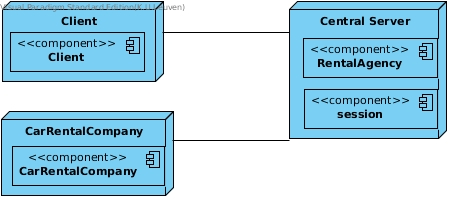
\includegraphics{deployment-diagram.jpg}

    \section{Sequence diagram}
    Sequence diagrams of the booking process have been included in the project.
    See 'sequence-diagram-success.jpg' and 'sequence-diagram-fail.jpg'.

    %    step  | client                     | agency                | crc
    %    1     | getNewReservationSession   | getRentalSession
    %    2.a   | checkForAvailableCarTypes  |                       | getAvailableCarTypes
    %    2.b   | addQuoteToSession(region1)
    %    2.c   | checkForAvailableCarTypes  |                       | getAvailableCarTypes
    %    2.d   | addQuoteToSession(region2)
    %    3     | confirmQuotes
    %    3.a.a |                            | confirmQuotes         | confirmQuote
    %    3.a.b |                            | confirmQuotes         | confirmQuote
    %    4.a   | clearSessions              | removeReservationSession
    %    3.b   |                            | confirmQuotes         | confirmQuote
    %    3.b.a |                            | confirmQuotes         | confirmQuote => ERROR
    %    3.b.c |                            | confirmQuotes         | cancelReservation
    %    4.b.a | throw ReservationException

\end{document}